%%%%%%%%%%%%%%%%%%%%%%%%%%%%%%%%%%%%%%%%%%%%%%%%%%%%%%%%%%%
% --------------------------------------------------------
% Tau
% LaTeX Template
% Version 2.4.4 (28/02/2025)
%
% Author: 
% Guillermo Jimenez (memo.notess1@gmail.com)
% 
% License:
% Creative Commons CC BY 4.0
% --------------------------------------------------------
%%%%%%%%%%%%%%%%%%%%%%%%%%%%%%%%%%%%%%%%%%%%%%%%%%%%%%%%%%%

\documentclass[10pt,letterpaper,onecolumn,report]{tau-class/tau}
\usepackage[english]{babel}
\usepackage{tabularx}
\usepackage{float}

%% Spanish babel recomendation
% \usepackage[spanish,es-nodecimaldot,es-noindentfirst]{babel} 

%----------------------------------------------------------
% TITLE
%----------------------------------------------------------

\journalname{Quantitative Engineering Analysis II}
\title{Unconstrained and Constrained Optimization on the Jungle Bridge}

%----------------------------------------------------------
% AUTHORS, AFFILIATIONS AND PROFESSOR
%----------------------------------------------------------

\author[1]{Tamás Regan}
\author[1]{Henry Tejada Deras}

%----------------------------------------------------------

\affil[1]{Franklin W. Olin College of Engineering}

%----------------------------------------------------------
% FOOTER INFORMATION
%----------------------------------------------------------

\institution{Franklin W. Olin College of Engineering}
\footinfo{Quantitative Engineering Analysis II}
\theday{April 14, 2025}
\leadauthor{Regan et al.}

%----------------------------------------------------------
% MAIN DOCUMENT
%----------------------------------------------------------

\begin{document}
		
    \maketitle 
    \thispagestyle{firststyle} 
    
%----------------------------------------------------------

\section{Overview and Introduction}

    The main goal of the Jungle Bridge project was to predict the shape of a bridge using constrained and unconstrained optimization, specifically with the gradient descent algorithm. For the unconstrained optimization aspect, we created a bridge made up of rubber band segments that could stretch as needed, and weights were placed on the ends of the segments to link them together. For the constrained optimization aspect, we followed a very similar approach, with the only change being that the bridge segments were now made up of string (which does not stretch as much as the rubber bands do, and thus we can assume that the segment lengths don’t change).

    In this project, we started off with the unconstrained optimization aspect. In order for us to use the gradient descent, we needed first to use linear regression to create an equation that would model the amount the rubber bands would stretch with respect to the weight that the rubber band would hold (and the resulting tension that it would cause). Now that we had an equation that represented that relationship, we needed to create another equation that would be used by the gradient descent algorithm to determine what the most stable shape for the bridge is. To do this, we created an equation that calculated the total potential energy of the bridge; in this case, it was adding both spring potential energy and gravitational potential energy for each segment. Then, we specified that we wanted the configuration that would have the least amount of potential energy as defined by the equation we just created (this is because, from our physics models, we know that all things in the universe naturally want to have the least amount of energy; we are assuming that there is no kinetic energy in the bridge). Finally, we ran the algorithm and it outputted the optimal shape of the bridge based on masses at the joints between the segments of the bridge, the relationship between mass held and length stretched for each of the rubber band segments, and the potential energy that the bridge would have for a given shape. For the constrained optimization aspect, we used almost the same algorithm as outlined above with the exception of a few modifications to account for our use of string instead of rubber bands. Since we used string (a material that, for our purposes, does not stretch at all), we know that its relationship between its length stretched to weight held (and its resulting tension) is that for every increase in weight held, the length stretched does not change. In addition, due to the previous relationship, we can now also model the total potential energy of the bridge as being only the gravitational potential energy per segment. This is because of the previous relationship stated and how that does not allow the segment to store any potential energy. One last thing, for our constrained optimization aspect, we also made all of the segment lengths static so it would better model the constraints of the bridge. Afterwards, we ran the gradient descent algorithm, taking everything listed above into account, and it outputted the ideal shape that would allow the bridge to be most stable.

\section{Methodology}

    \subsection{Jungle Bridge (Rubber Band) Physical Model Characteristics}

        The Jungle Bridge we made comprised 6 rubber bands of varying lengths and 5 weights that were used to hold the rubber bands together at the ends of each segment. The weights used varied in weight (see Table 4) along with the stiffness of the rubber band segments (see Table 2).

        \begin{table}[H]
            \centering
            \setcounter{table}{3} % Listed as 3 so when file is run, it is listed as table 4.
            \begin{tabular}{cc}
                 Weight Label & Weight (g)\\
                 1 (Pink) & 40\\
                 2 (Red) & 25\\
                 3 (Yellow 1) & 50\\
                 4 (Light Blue) & 50\\
                 5 (Yellow 2) & 50\\
            \end{tabular}
            \caption{Weights used in the jungle bridge model vertices.}
            \label{tab:4}
        \end{table}

        To calculate the stiffness of the rubber band segments, we hung different weights from each rubber band and measured how much each rubber band stretched. We recorded our data in Table 1.

        
        \begin{table}[H]
            \centering
            \setcounter{table}{0} % Listed as 0 so when file is run, it is listed as table 1.
            \resizebox{\textwidth}{!}{
            \begin{tabular}{lllllcc}
             & \multicolumn{2}{c}{Rubber Band \#1 - Light Green}& \multicolumn{2}{c}{Rubber Band \#2 - Dark Blue}&\multicolumn{2}{c}{Rubber Band \#3 - Orange}\\
             & Mass (g)&Stretched Length (cm)& Mass (g)&Stretched Length (cm)&Mass (g)&  Stretched Length (cm)\\
             Measurement 1& 20& 11.75& 22& 8.25& 21& 8.5\\
             Measurement 2& 40& 12.25& 42& 8.25& 63& 8.75\\
             Measurement 3& 62& 12.25& 63& 8.75& 61& 8.75\\
             Measurement 4& 83& 12.5& 103& 9& 81& 9\\
             Untensed Measurement& 0& 10.5& 0& 7.25& 0& 7.25\\
             & & & & & &\\
             & \multicolumn{2}{c}{Rubber Band \#4 - Rust Red}& \multicolumn{2}{c}{Rubber Band \#5 - Dusty Red}& \multicolumn{2}{c}{Rubber Band \#6 - Light Brown}\\
             & Mass (g)& Stretched Length (cm)& Mass (g)& Stretched Length (cm)& Mass (g)& Stretched Length (cm)\\
             Measurement 1
             & 20& 6.25& 22& 6.25& 20&9\\
             Measurement 2
             & 40& 6.5& 42& 6.75& 42&9.5\\
             Measurement 3
             & 62& 6.5& 82& 6.75& 62&10\\
             Measurement 4
             & 103& 6.75& 103& 7& 83&10.25\\
             Untensed Measurement& 0& 4.75& 0& 5.5& 0&7.25\\
            \end{tabular}
            }
            \caption{Measurements used to calculate the stiffness and natural length of each rubber band used in the jungle bridge model.}
            \label{tab:my_label}
        \end{table}   

        Using the measurements above, we computed the stiffness and natural length of each rubber band using simple linear regression.      

        \begin{equation}
            \begin{bmatrix}
            m^*\\
            b^*
            \end{bmatrix}
            =(A^TA)^{-1}A^TY
        \end{equation}

        In order to do this, we need to prepare two different matrices, one matrix, \(\textbf{A}\) is comprised of the length that the rubber band stretched under different weights in one column and the number \(1\) in the other column.

        \begin{equation}
            \textbf{A} =
            \begin{bmatrix}
            l_1 & 1\\
            l_2 & 1\\
            \vdots & \vdots\\
            l_n & 1\\
            \end{bmatrix}
        \end{equation}

        The reason matrix \(\textbf{A}\) is set up this way is because this matrix will store the basis vectors of the data, and in this way, encoding the \(x\) values of the data. The other matrix, \(\textbf{Y}\) is a column vector with the gravitational force exerted by the mass hanging from the rubber band, calculated by using Newton’s second law.

        \begin{equation}
            \textbf{Y} =
            \begin{bmatrix}
            F_1\\
            F_2\\
            \vdots\\
            F_n\\
            \end{bmatrix}
            =
            \begin{bmatrix}
            m_1 \cdot g\\
            m_2 \cdot g\\
            \vdots\\
            m_n \cdot g\\
            \end{bmatrix}
        \end{equation}        

        This process finds the sum of the squared distances between the measured points (in other words, the error in the predictions made by the line of best fit) and the line of best fit and then minimizes that sum of the squared distances to make the most accurate line of best fit based on the data. This in of itself is another form of optimization problem in which our objective is to minimize the error between the measured data and the line of best fit.

        \begin{equation}
            \min_{(m, b)}E(m, b) = ((m\textbf{X}+b\textbf{1})-\textbf{Y})^2
        \end{equation}
        
        \begin{figure}[H]
            \centering
            \setcounter{figure}{1} % Listed as 1 so when file is run, it is listed as figure 2.
            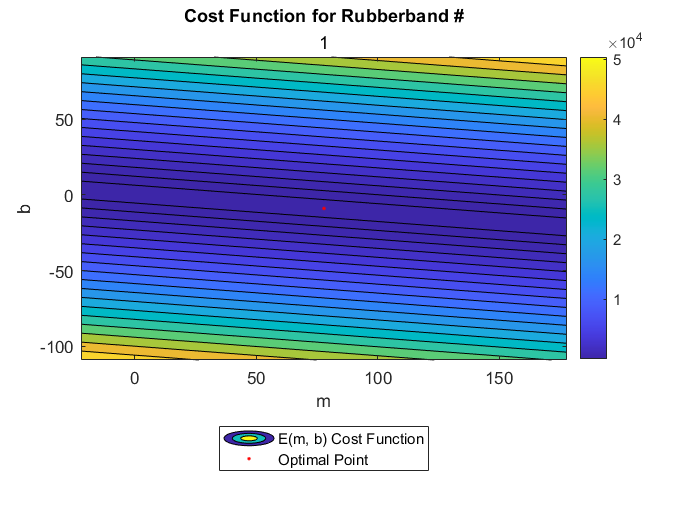
\includegraphics[width=0.5\linewidth]{figures/figure 2; cost function rubber band 1.png}
            \caption{Optimal Point in the perspective of the objective function for rubber band \#1.}
            \label{fig:enter-label}
        \end{figure}
        
        In the end, we get a line of best fit based on our data, which we can use along with Hooke’s law to extract the stiffness, \(k\), and natural length, \(l_0\), for each rubber band.

        \begin{figure}[H]
            \centering
            \setcounter{figure}{0} % Listed as 0 so when file is run, it is listed as figure 1.
            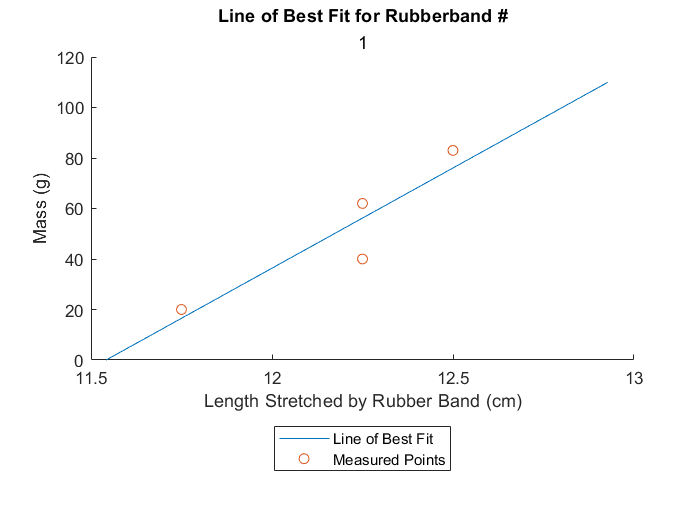
\includegraphics[width=0.5\linewidth]{figures/figure 1; line of best fit rubber band 1.png}
            \caption{Line of best fit for rubber band \#1}
            \label{fig:enter-label}
        \end{figure}

        Using that, we can easily translate the slope and \(y\)-intercept of the line to stiffness, \(k\), and natural length, \(l_0\), values for each rubber band.

        \begin{equation}
            F=ml + b = k(l-l_0) = kl - kl_0 \Rightarrow k = m; l_0 = \frac {-b} {m}
        \end{equation}

        After all of that, we have arrived at the following calculated values. These values will be used to characterize the behavior of the rubber bands under different weights and will be used to calculate the shape of the jungle bridge.
        
        \begin{table}[H]
            \centering
            \setcounter{table}{1} % Listed as 1 so when file is run, it is listed as table 2.
            \begin{tabular}{ccc}
                 &  \(k\) - Stiffness (N/m)& \(l_0\) - Natural Length (m)\\
                 Rubber Band 1 - Light Green
                &  77.78105263158126
                & 0.11541777188328932
                \\
                 Rubber Band 2 - Dark Blue
                &  85.65925925926581
                & 0.07904661016949203
                \\
                 Rubber Band 3 - Orange
                &  117.59999999998126
                & 0.08324999999999931
                \\
                 Rubber Band 4 - Rust Red
                &  162.6800000000284
                & 0.06161144578313313
                \\
                 Rubber Band 5 - Dusty Red
                &  100.06315789472805
                & 0.06077835051546339
                \\
                 Rubber Band 6 - Light Brown
                &  47.23932203389761
                & 0.08613924050632896
                \\
            \end{tabular}
            \caption{Stiffness and Natural Length calculations based on running a linear regression algorithm on the data collected.}
            \label{tab:my_label}
        \end{table}

        The physical model we built looks as follows (Figure 3), with vertex measurements in the following table (Table 3).

        \begin{figure}[H]
            \centering
            \setcounter{figure}{2} % Listed as 2 so when file is run, it is listed as figure 3.
            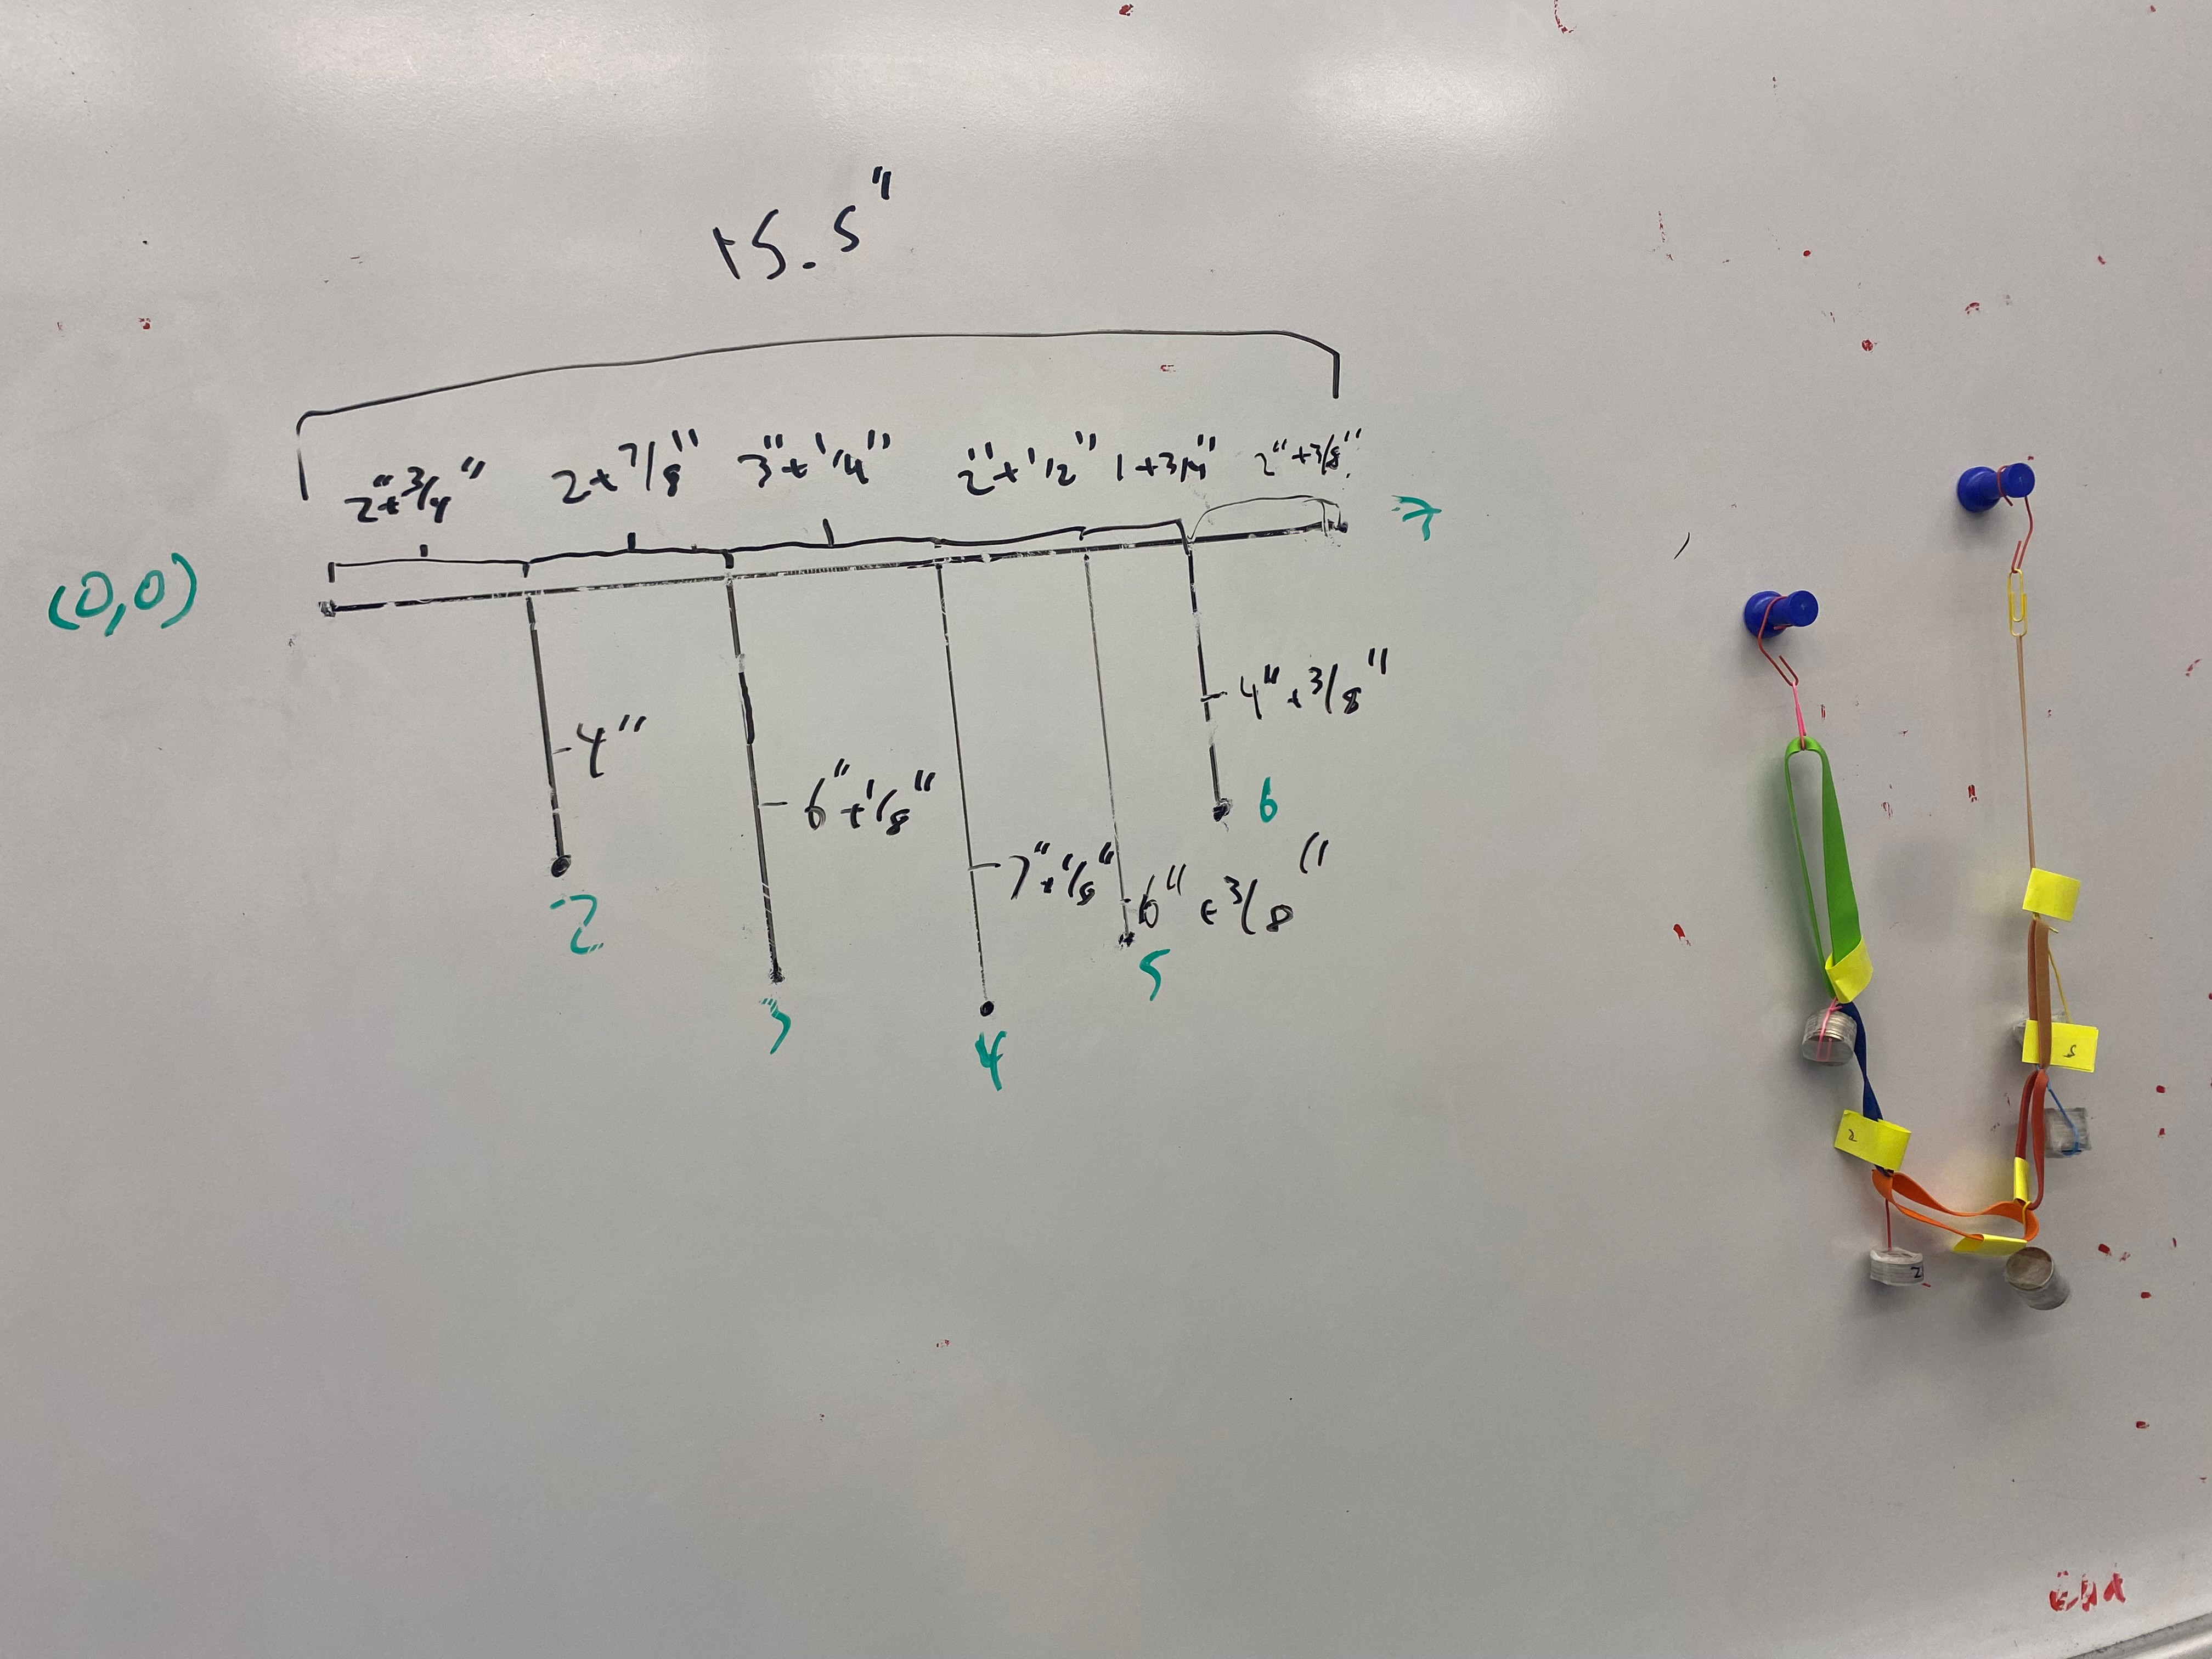
\includegraphics[width=0.5\linewidth]{figures/figure 3; jungle bridge.jpg}
            \caption{Physical Jungle Bridge Model. The physical model is to the side while the vertex measurements are in the center.}
            \label{fig:enter-label}
        \end{figure}
        
        \begin{table}[H]
            \centering
            \setcounter{table}{2} % Listed as 2 so when file is run, it is listed as table 3.
            \begin{tabular}{ccc}
                 Coordinate Label
                &  \(x\) Coordinate (cm)
                & \(y\) Coordinate (cm)
                \\
                                 1 (Left Vertex)
                &  0
                & 0
                \\
                                 2 (Weight 1 Vertex)
                &  6.985
                & -10.16
                \\
                                 3 (Weight 2 Vertex)
                &  14.2875
                & -15.5575
                \\
                                 4 (Weight 3 Vertex)
                &  22.5425
                & -18.0975
                \\
                                 5 (Weight 4 Vertex)
                &  28.8925
                & -16.1925
                \\
                                 6 (Weight 5 Vertex)
                &  33.3375
                & -11.1125
                \\
                                 7 (Right Vertex)
                &  39.37
                & 0
                \\
            \end{tabular}
            \caption{Coordinate description of the location of the jungle bridge’s vertices based on the leftmost vertex being the origin.}
            \label{tab:my_label}
        \end{table}
    
    \subsection{Unconstrained Optimization}

        Before we can use gradient descent to solve this unconstrained optimization problem, we first need to define what a gradient is and how to compute it numerically. A gradient, represented by the symbol Nabla (\(\nabla\)), is an operator on a function (in other words, it does something to a function) that stores all the partial derivatives of the function in every dimension. Think of this as a container for all of these partial derivatives.

        \begin{equation}
            \nabla f(x) = 
            \begin{bmatrix}
                \frac {\partial f} {\partial x_1} \\
                \vdots \\
                \frac {\partial f} {\partial x_n} \\
            \end{bmatrix}
            \text{ where } p = (x_1, \ldots, x_n)
        \end{equation}

        What this represents with all of these partial derivatives is how the surface created by a multi-variable equation is changing in every direction. Numerically speaking, we would calculate the partial derivatives of the multi-variable function and then plug in the relevant coordinates to get how much the surface is changing in a direction. In practice, it would look similar to this given the multi-variable function \(f(x,y) = x^2 + 2xy^2\) and the point \((1, 0)\) at which you are trying to find the gradient at. First, you would approximate the partial derivatives by evaluating the function at two different points, separated by a very small step size, \(h\), along one direction.

        \begin{equation}
            \frac {\partial f} {\partial x} = \frac {f(x + h, y) - f(x, y)} {h} \text{; } \frac{\partial f}{\partial y} = \frac{f(x, y + h) - f(x, y)}{h}
        \end{equation}

        Next, you would assemble these partial derivatives into the gradient which would be as follows.

        \begin{equation}
            \nabla f\left(x,\ y\right)=\left[\begin{matrix}\frac{\partial f}{\partial x}\\\frac{\partial f}{\partial y}\\\end{matrix}\right]=\left[\begin{matrix}\frac{f\left(x+h,\ y\right)-f(x,\ y)}{h}\\\frac{f\left(x,\ y+h\right)-f(x,\ y)}{h}\\\end{matrix}\right]=\left[\begin{matrix}\left[{(x+h)}^2+2(x+h)y^2\right]-\left[x^2+2xy^2\right]\\\left[x^2+2x\left(y+h\right)^2\right]-\left[x^2+2xy^2\right]\\\end{matrix}\right]
        \end{equation}

        Then you would plug in the \(x\) and \(y\) values into the gradient of the function and solve. In this example, that would look as follows. Note: The number of variables you would use would depend on the number of variables your function has. Since this function has two variables, we only need to use two variables.

        \begin{equation}
            \nabla f\left(1,\ 0\right)=\left[\begin{matrix}\frac{\left[{(1+1^{-5})}^2+2(1+1^{-5})0^2\right]-\left[1^2+2(1)0^2\right]}{1^{-5}}\\\frac{\left[1^2+2(1)\left(0+1^{-5}\right)^2\right]-\left[1^2+2(1)0^2\right]}{1^{-5}}\\\end{matrix}\right]\approx\left[\begin{matrix}2\\0\\\end{matrix}\right]
        \end{equation}

        We can interpret this outcome as the surface is changing in \(y\)-direction but not changing in the \(x\)-direction based on the values of each partial derivative component. This matches what the surface looks like, the surface is changing if you move in the y-direction, but not if you move in the \(x\)-direction.

        \begin{figure}[H]
            \centering
            \setcounter{figure}{7} % Listed as 7 so when file is run, it is listed as figure 8.
            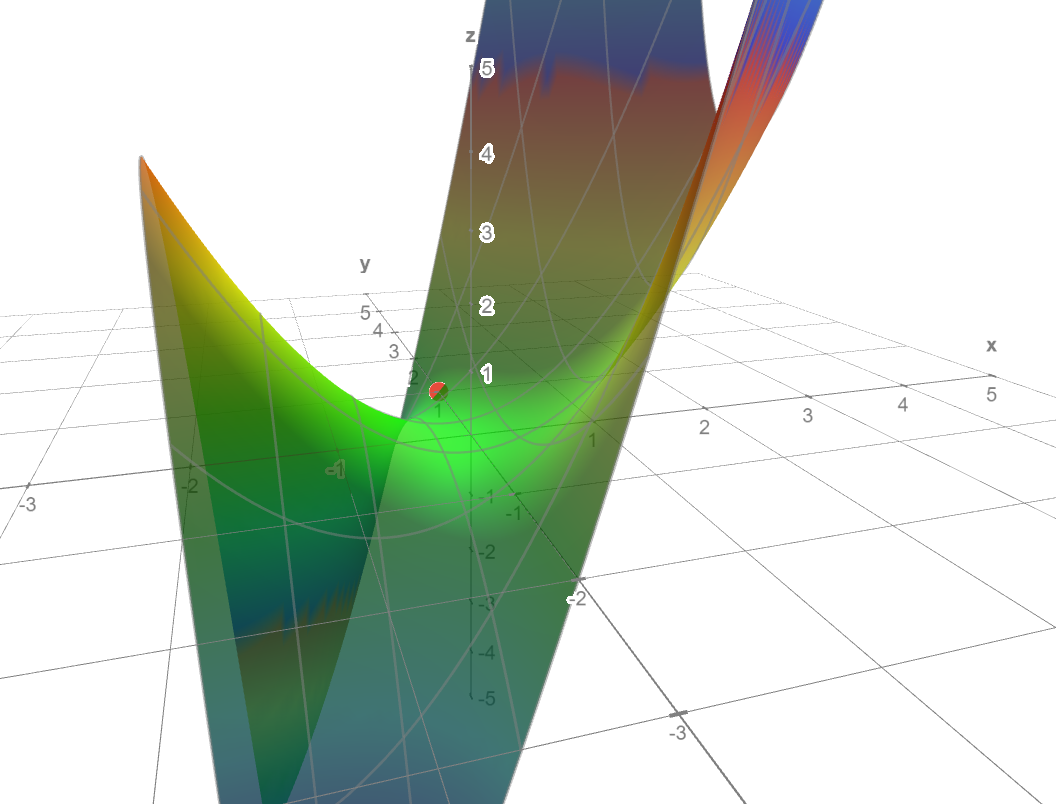
\includegraphics[width=0.5\linewidth]{figures/example curve.png}
            \caption{$x^2 + 2xy^2$ plotted on Math 3D with the point $(0, 1, 0)$ plotted in red.}
            \label{fig:enter-label}
        \end{figure}

        Now we can begin the gradient descent algorithm to solve this unconstrained optimization problem. This algorithm uses a nuanced property of the gradient which is that the gradient will always point in the direction of the steepest ascent. This is true because the gradient is always perpendicular to the contour lines (or equivalent) of a multi-variable function and is therefore moving the quickest away from the point at which the gradient was calculated.

        The gradient descent algorithm has 5 steps, not including the number of times you would iterate through a set of steps. Before starting, you will need to define an objective function (which is a relationship between the variables that you can change in your problem and the outcome of those variables) and a step size for the algorithm (this will be explained later). First, you determine whether you want to find the minimum or maximum of the objective function you have. In the case of our jungle bridge problem, it is as follows:

        \begin{equation}
            \min U_{total}(m_i, l_i) \text{ where } U_{total}(m_i, l_i)= \sum_{i = 1}^{n} gm_{i}y_{i} + \sum_{i = }^{n} \frac {1} {2} k_{i} (\max(l_i - l_0))^2 \text{ and } l_i = \sqrt{(x_{i + 1} - x_i)^2 + (y_{i + 1} - y_i)^2}
        \end{equation}

        The reason the objective function we chose is as listed above is because the most likely shape of the jungle bridge would be that of when it is most at rest (given that the left and right vertices are fixed in this problem). Therefore, the objective function that we will use (as seen above) is one that calculates the total potential energy stored by the bridge which is only gravitational and elastic potential energy. In addition, we also specifically are looking for the minimum of the objective function since the bridge will be most at rest the less potential energy it has.

        Next, we will select a random point and compute the gradient at that point. After that, we will check if the gradient at that point is equal to 0. This is important because if the gradient is equal to 0 (or something very close to it), that means we have found our most optimal point for the given objective function. If the gradient is equal to 0 (or something very close to it), then that is your answer; if not, multiply the gradient vector by some step size (preferably on the smaller side so the gradient descent algorithm does not pass up the optimal point) you defined before starting the gradient descent algorithm. This step size parameter is used to regulate how much the initial point changes when it is multiplied by the previous point. After you multiply the gradient vector by the step size parameter, you will multiply that vector by the previous point output by the gradient descent algorithm (if this is the first iteration through this loop, this will be your initial guess). What you are doing in this step is essentially taking one step on the path you are creating while “going down the hill” that is the surface of the multi-variable objective function in order to find the lowest point (or the minimum) in this problem. Then, you calculate the gradient at this new point output by the gradient descent algorithm and repeat steps 3-5 as many times as you would like or until you reach the optimal point.

        \begin{figure}[H]
            \centering
            \setcounter{figure}{8} % Listed as 8 so when file is run, it is listed as figure 9.
            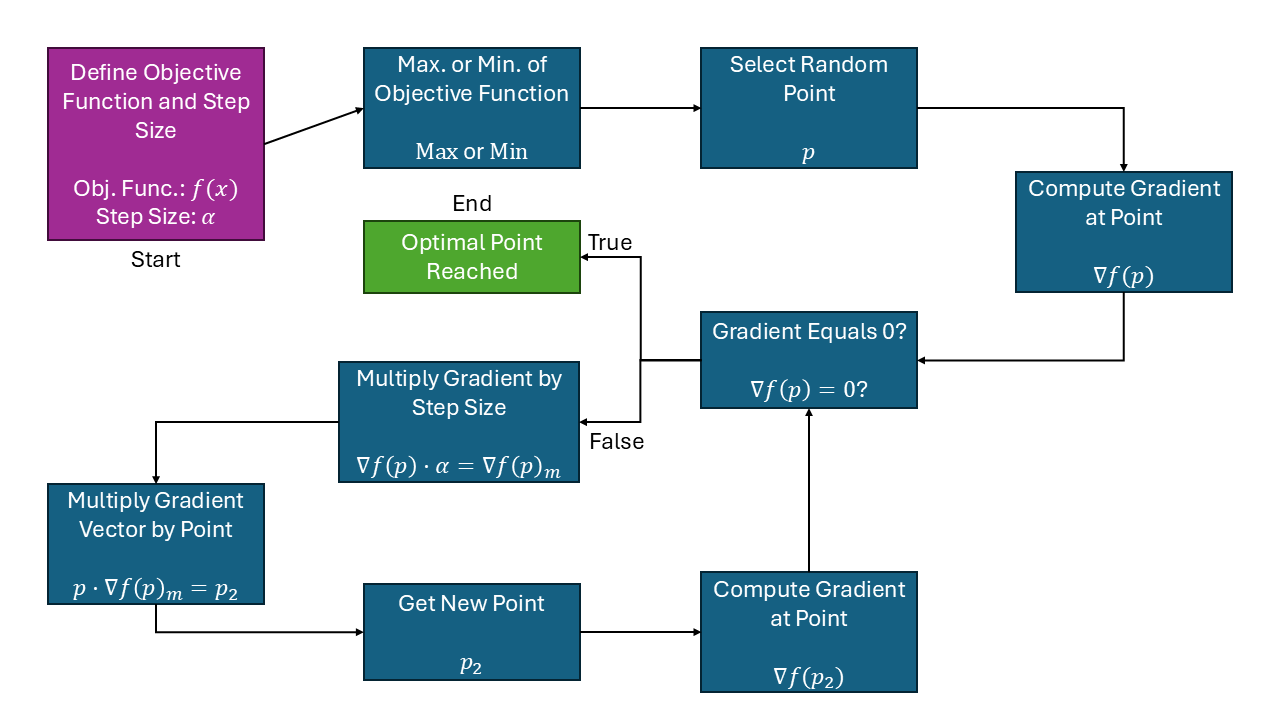
\includegraphics[width=0.5\linewidth]{figures/Gradient Descent Process Diagram.png}
            \caption{Gradient Descent Process Flowchart}
            \label{fig:enter-label}
        \end{figure}

        For this problem specifically, we followed the gradient descent algorithm with a small modification. We added the backtracking line search algorithm to adjust the step size parameter dynamically as we are running the gradient descent algorithm. This is intended to help fix the issue with the gradient descent algorithm passing up the most optimal point (or never reaching it due to a step size that is too large). This algorithm changes the step size parameter based on the size of the gradient vector at that iteration’s point. If the gradient vector is large, then the step size will also be large and vice versa.

        In our implementation, we iterated through the gradient descent algorithm 1000 times using the backtracking line search algorithm. Below is a visualization of this process.

        \begin{figure}[H]
            \centering
            \setcounter{figure}{4} % Listed as 4 so when file is run, it is listed as figure 5.
            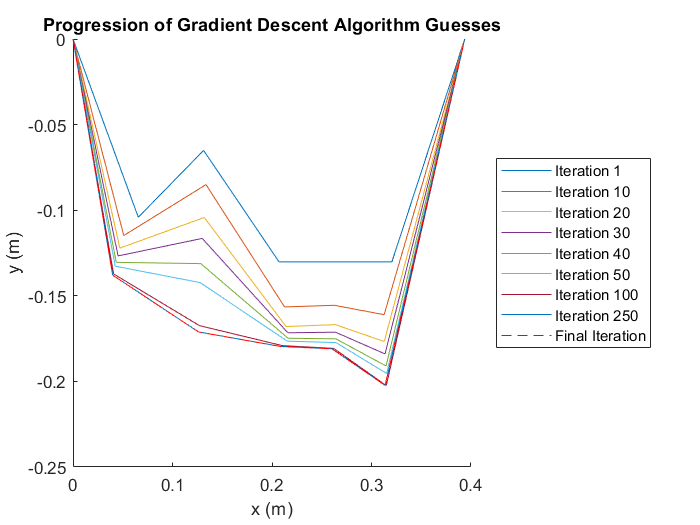
\includegraphics[width=0.5\linewidth]{figures/figure 5; gradient descent progression.png}
            \caption{Progression of Gradient Descent Algorithm Guesses by Iteration}
            \label{fig:enter-label}
        \end{figure}

    \subsection{Rope Bridge Physical Model Characteristics}

        For our rope bridge model, it was comprised of 6 string segments with 5 weights hanging from the middle vertices of the bridge. The left and right vertices were affixed to their respective points.

        \begin{figure}
            \centering
            \includegraphics[width=0.5\linewidth]{figures/figure 4; rope bridge.jpg}
            \caption{Rope Bridge Physical Model with Tamás posing for the photo.}
            \label{fig:enter-label}
        \end{figure}

        The segment lengths were measured before building the bridge and are as follows.
        
        \begin{table}[H]
            \centering
            \setcounter{table}{4} % Listed as 4 so when file is run, it is listed as table 5.
            \begin{tabular}{ccc}
                 Segment Name
                &  Coordinate Labels
                & Length (cm)
                \\
                                 1
                &  0 to 1
                & 19
                \\
                                 2
                &  1 to 2
                & 19.8
                \\
                                 3
                &  2 to 3
                & 15
                \\
                                 4
                &  3 to 4
                & 15.7
                \\
                                 5
                &  4 to 5
                & 10.7
                \\
                                 6
                &  5 to 6
                & 3.5
                \\
            \end{tabular}
            \caption{Measured lengths of rope bridge segments.}
            \label{tab:my_label}
        \end{table}

        The weights used on the bridge were also measured and are as follows.
        
        \begin{table}[H]
            \centering
            \setcounter{table}{5} % Listed as 5 so when file is run, it is listed as table 6.
            \begin{tabular}{cc}
                 Weight Label& Mass (g)\\
                 1& 26\\
                 2& 41\\
                 3& 25\\
                 4& 51\\
                 5& 41\\
            \end{tabular}
            \caption{Weight measurements of weights hung from rope bridge vertices.}
            \label{tab:my_label}
        \end{table}

        After the bridge was built, we measured the positions of the bridge vertices with respect to the left most vertex which we defined as the origin of the coordinate system. The measurements are as follows.
        
        \begin{table}[H]
            \centering
            \setcounter{table}{6} % Listed as 6 so when file is run, it is listed as table 7.
            \begin{tabular}{ccc}
                 Coordinate Label&  x Coordinate (cm)& y Coordinate (cm)\\
                 0 (Left Vertex)&  0& 0\\
                 1 (Weight 1 Vertex)&  25.7& -12.2\\
                 2 (Weight 2 Vertex)&  44.4& -17.1\\
                 3 (Weight 3 Vertex)&  59.6& -16.8\\
                 4 (Weight 4 Vertex)&  75.2& -13\\
                 5 (Weight 5 Vertex)&  84.3& -7\\
                 6 (Right Vertex)&  91.8& 0\\
            \end{tabular}
            \caption{Measured coordinate locations of the rope bridge vertices.}
            \label{tab:my_label}
        \end{table}

    \subsection{Constrained Optimization}

        Since the segments were made of string, that adds a constraint to our problem and changes it to a constrained optimization problem. The segments being made of string add a constraint to the length of the segments. This is because a string does not stretch any meaningful amount under any load (except when it breaks) and therefore has an infinite stiffness value. Mathematically speaking, this causes the natural length of the segment to be the only length that the segment can be, it cannot be more as that would represent the segment breaking and it cannot be less since that would not make sense for a bridge that is suspended in air without any supports in any of the segments and is under strain by the weights placed on its middle vertices. The constraint is summed up as follows.

        \begin{equation}
            \text{s.t. } l = l_0
        \end{equation}

        \(l\) is defined as the length of the string and \(l_0\) is defined as the natural length of the string.
        
        Now, to solve this problem, we will use a process very different from the one used in the unconstrained optimization problem. Since we have constraints, we need to make sure the optimal point fits the constraints. To do this, we need a special property.

        \begin{equation}
            \nabla f(x) + \lambda \nabla g(x) = 0
            \text{ where } x \text{ is a point and } g(x) \text{ is a constraint equation}
        \end{equation}

        This property is saying that for a point(s) when the gradient of the objective function points in the same direction as the gradient all of the constraint equations combined multiplied by their respective LaGrange multipliers (which are just numbers that are multiplied by the gradient of the constraint equations to make the gradients equal in magnitude), then that is equal to 0. This is very useful because, in practice, when this property is true, that point is the minimum point of the objective function taking into account the constraints on the objective function. Using this information, we will then construct a new equation that uses this property to take into account the constraints of the objective function and the objective function itself, and convert this problem into an unconstrained optimization problem. This is how it would look in the form of an equation.

        \begin{equation}
            F^*(x_1, \ldots, x_n, \lambda_1, \ldots, \lambda_n) = f(x_1, \ldots, x_n, \lambda_1, \ldots, \lambda_n) + \sum_{i=1}^n \lambda_i g(x_1, \ldots, x_n, \lambda_1, \ldots, \lambda_n)
        \end{equation}

        With this equation, we cannot just run the gradient descent algorithm as we did before; the points at which the property above is true are saddle points. If we ran the gradient descent algorithm, the algorithm would go towards infinity and never stop at any of these points since it is looking for a minimum point, not a saddle point. Instead, we need to find the critical points of the new function, \(F^*\), and the point that gives the smallest output of the function would be the most optimal point for our problem. In our problem, we did this section by using MATLAB’s fmincon function.
        
        \begin{lstlisting}[language=Matlab, caption=Using fmincon to compute the most optimal point from our modified objective function (taking into account the constraints).]
            % use fmincon to compute the predicted vertex locations
            coords_sol = fmincon(f_cost, coords_guess, [], [], [], [], [], [], f_cstr);
        \end{lstlisting}

        Though, as a side note, you can run the unconstrained gradient descent model from above to model the string bridge by making the natural lengths the lengths of the strings and the stiffness values infinity. We did not decide to use this approach, but it is another valid way of modeling the string bridge.

    \subsection{Difference between Constrained and Unconstrained Optimization}

        The main difference between constrained and unconstrained optimization is that, as the name implies, one has constraints while the other does not. In practice, the way that you solve these problems is very different. To solve unconstrained optimization problems, you can use the gradient descent algorithm and find the minimum of the objective function (or the maximum if you multiply the gradient by -1). To solve constrained optimization problems, you have to take into account the problem’s constraints and create a modified objective function that includes the constraints; afterwards, you find the critical points of the modified objective function and then solve for the output of the objective function to determine which of those points is the minimum based on the output of the objective function. When you do this process, you convert the problem to an unconstrained optimization problem, but you do not solve it like an unconstrained optimization problem due to the saddle points. In short, the process to solve the constrained and unconstrained optimization problems is very different.
        
\section{Results}
    \subsection{Unconstrained Optimization Result}
    
        \begin{figure}[H]
            \centering
            \setcounter{figure}{5} % Listed as 5 so when file is run, it is listed as figure 6.
            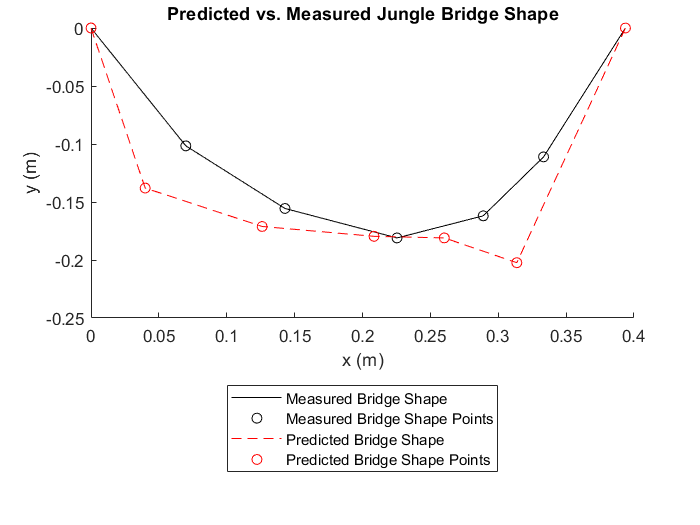
\includegraphics[width=0.5\linewidth]{figures/figure 6; measured vs. predicted jungle bridge shape.png}
            \caption{Comparison of Measured vs. Predicted Jungle Bridge Shape}
            \label{fig:enter-label}
        \end{figure}
        
        As you can see, the predicted is not the same as the measured, specifically, there are differences in the shape of the bridge made. This is probably due to our measurement errors, which are discussed in more detail in the interpretation section.
        
    \subsection{Constrained Optimization Result}
        
        \begin{figure}
            \centering
            \setcounter{figure}{6} % Listed as 6 so when file is run, it is listed as figure 7.
            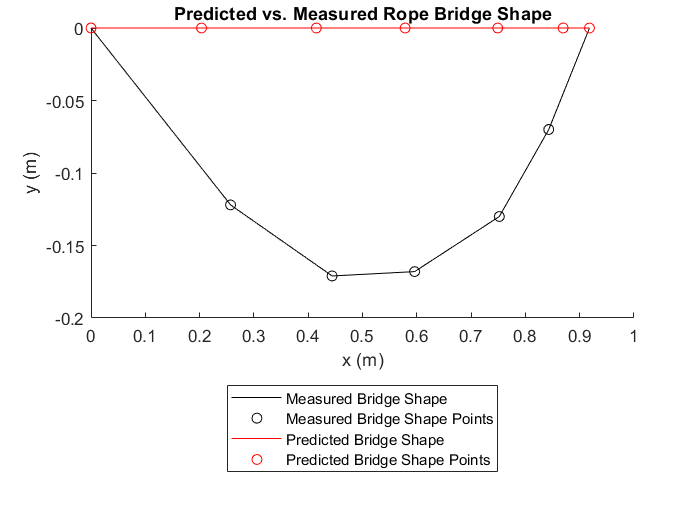
\includegraphics[width=0.5\linewidth]{figures/figure 7; measured vs. predicted rope bridge shape.png}
            \caption{Comparison of Measured vs. Predicted Rope Bridge Shape}
            \label{fig:enter-label}
        \end{figure}
                
        As you can see, this graph does not at all line up with the measured graph. The reasons for this are unknown to us. We took this problem to Olivia Smith (a QEA II CA), and we could not figure out why this was happening.

\section{Interpretation}
    The reason that optimizing the potential energy function of the system allows us to predict the shape of both bridges with some accuracy is because the final shape of the bridge after we set it up is at rest. The system wants to minimize its potential energy (The bridge wants to fall, the rubber bands want to contract back to their natural length), so minimizing the function that represents the total potential energy allows us to use the x and y coordinates of the vertices that best minimize the function as appropriate guesses at what they would be in real life.
    
    However, our model was not completely accurate, and that means there was some error in our model. Listed here are the potential sources that we could think of (All of which were measurement errors:
    
    Measurement Errors:
    
    \begin{itemize}
        \item \(k\) value measurements
            \begin{itemize}
                \item Length of stretched rubber bands
            \end{itemize}
            \begin{itemize}
                \item Mass of weights
            \end{itemize}
        \item Error in measuring string lengths
        \item Error in measuring distances between joints of our bridge on a whiteboard
    \end{itemize}

    Biggest Errors:
    
    \begin{itemize}
        \item Measurement of stretched rubber band lengths (Because this was done ad hock by holding up a ruler and hanging our stretched rubber band next to it.)
        \item Measurement of join locations (The measurements of the locations were all dependent on one point on the board being (0,0), so the error in the early measurement's compounds with the error in the measurements farther away from the origin point
    \end{itemize}
    
    We might make this error better in the future by overlaying our jungle bridge over a coordinate grid, reducing the compounding error, as well as tape the ruler to a wall that we use to measure stretched length so that we are not simultaneously holding the rubber band and the ruler.

\section{Team Attribution Statement}

We are a group comprised of Tamás Regan and Henry Tejada Deras. Tamás focused on most of the methodology and conceptual sections of the report, debugging code, writing various parts of the report, and writing pseudocode to make the gradient descent algorithm work. Henry focused on writing Tamás’ pseudocode into MATLAB code, debugging the code, and writing the other parts of the report. A special thank you goes to Althea Ivins and Jacob Likins, who helped us debug our code.

\end{document}